% ============================================================
%  RAPPORT DE PROJET --- MedBox Recognition API
%  Master Informatique et Technologies --- UM5 FSR Rabat
%  Bin\^ome : Chaymae / Wiam | Juin 2026
% ============================================================
\documentclass[12pt,a4paper]{report}

% - Encodage & langues -
\usepackage[utf8]{inputenc}
\usepackage[T1]{fontenc}
\usepackage[french]{babel}



% - Mise en page -
\usepackage[top=2.5cm,bottom=2.5cm,left=2.8cm,right=2.5cm]{geometry}
\usepackage{fancyhdr}
\usepackage{emptypage}
\usepackage{titlesec}
\usepackage{titletoc}
\usepackage{setspace}
\usepackage{parskip}

% - Couleurs -
\usepackage[dvipsnames,table]{xcolor}
\definecolor{primary}{RGB}{27,94,56}
\definecolor{secondary}{RGB}{46,125,82}
\definecolor{accent}{RGB}{76,175,132}
\definecolor{success}{RGB}{27,94,56}
\definecolor{warning}{RGB}{255,165,0}
\definecolor{danger}{RGB}{192,0,0}
\definecolor{lightgray}{RGB}{245,245,245}
\definecolor{darkgray}{RGB}{80,80,80}
\definecolor{codebg}{RGB}{232,245,238}
\definecolor{teal}{RGB}{46,125,82}

% - Graphiques & figures -
\usepackage{graphicx}
\usepackage{float}
\usepackage{wrapfig}
\usepackage{subcaption}
\usepackage{tikz}
\usetikzlibrary{shapes.geometric, arrows.meta, positioning, fit, backgrounds, shadows}

% - Tableaux -
\usepackage{booktabs}
\usepackage{tabularx}
\usepackage{multirow}
\usepackage{longtable}
\usepackage{array}
\usepackage{colortbl}

% - Math\'ematiques -
\usepackage{amsmath}
\usepackage{amssymb}

% - Code source -
\usepackage{listings}
\lstset{
  backgroundcolor=\color{codebg},
  basicstyle=\ttfamily\footnotesize,
  breaklines=true,
  frame=single,
  rulecolor=\color{secondary!40},
  numbers=left,
  numberstyle=\tiny\color{gray},
  keywordstyle=\color{primary}\bfseries,
  commentstyle=\color{success}\itshape,
  stringstyle=\color{accent},
  xleftmargin=15pt,
  xrightmargin=5pt,
  captionpos=b,
  showstringspaces=false,
}
\lstdefinelanguage{Python}{
  keywords={def,class,import,from,return,if,elif,else,for,while,try,except,with,as,in,not,and,or,True,False,None,self,lambda},
  morestring=[b]",
  morestring=[b]',
  morecomment=[l]{\#},
}

% - Bo\^ites color\'ees -
\usepackage[most]{tcolorbox}
\tcbuselibrary{breakable,skins}

\newtcolorbox{infobox}[1][]{
  colback=secondary!8, colframe=secondary,
  fonttitle=\bfseries\small, title=#1,
  arc=4pt, boxrule=0.8pt, left=8pt, right=8pt,
  top=6pt, bottom=6pt, breakable
}
\newtcolorbox{successbox}[1][]{
  colback=success!8, colframe=success,
  fonttitle=\bfseries\small, title=#1,
  arc=4pt, boxrule=0.8pt, left=8pt, right=8pt,
  top=6pt, bottom=6pt, breakable
}
\newtcolorbox{warningbox}[1][]{
  colback=warning!10, colframe=warning,
  fonttitle=\bfseries\small, title=#1,
  arc=4pt, boxrule=0.8pt, left=8pt, right=8pt,
  top=6pt, bottom=6pt, breakable
}
\newtcolorbox{codebox}[1][]{
  colback=codebg, colframe=primary!40,
  fonttitle=\bfseries\small\color{primary}, title=#1,
  arc=4pt, boxrule=0.6pt, left=6pt, right=6pt,
  top=4pt, bottom=4pt, breakable
}

% - Liens hypertexte -
\usepackage[hidelinks,colorlinks=false]{hyperref}

% - Divers -
\usepackage{enumitem}
\usepackage{footnote}
\usepackage{caption}
\usepackage{microtype}
\usepackage{lmodern}
\usepackage{palatino}
\usepackage{mathpazo}

% - En-t\^etes et pieds de page -
\pagestyle{fancy}
\fancyhf{}
\fancyhead[L]{\small\color{darkgray}\textit{MedBox Recognition API}}
\fancyhead[R]{\small\color{darkgray}\textit{Master IT 2025--2026}}
\fancyfoot[C]{\small\color{darkgray}\thepage}
\renewcommand{\headrulewidth}{0.4pt}
\renewcommand{\footrulewidth}{0pt}

% - Styles de sections -
\titleformat{\chapter}[display]
  {\normalfont\huge\bfseries\color{primary}}
  {\chaptertitlename\ \thechapter}{20pt}{\Huge}
\titleformat{\section}
  {\normalfont\Large\bfseries\color{secondary}}
  {\thesection}{1em}{}
\titleformat{\subsection}
  {\normalfont\large\bfseries\color{darkgray}}
  {\thesubsection}{1em}{}

% - Commandes utilitaires -
\newcommand{\medbox}{\textsc{MedBox}\xspace}
\newcommand{\en}[1]{\textit{\textit{#1}}}
\newcommand{\code}[1]{\texttt{\small #1}}

% ============================================================
\begin{document}


% - Page de titre -
\begin{titlepage}
\pagecolor{white}
\centering
\vspace*{0.5cm}

{\color{primary}\rule{\linewidth}{2pt}}
\vspace{0.3cm}

{\large\bfseries Universit\'e Mohammed V -- Rabat}\\[0.2cm]
{\large Facult\'e des Sciences -- FSR}\\[0.1cm]
{\normalsize Master Informatique et Technologies (IT)}\\[0.1cm]
{\normalsize Ann\'ee acad\'emique 2025--2026}

\vspace{0.4cm}
{\color{primary}\rule{\linewidth}{0.8pt}}
\vspace{1cm}

\begin{tcolorbox}[colback=primary!5,colframe=primary,arc=8pt,boxrule=1.5pt]
\centering
{\LARGE\bfseries\color{primary} Rapport de Projet}\\[0.4cm]
{\huge\bfseries Medication Box Recognition API}\\[0.3cm]
{\large\color{secondary} Reconnaissance de Bo\^ites de M\'edicaments\\par Vision par Ordinateur et OCR}\\[0.2cm]
{\normalsize\color{darkgray}\en{Computer Vision-based Medication Identification System}}
\end{tcolorbox}

\vspace{0.8cm}

\begin{tikzpicture}[node distance=1.2cm]
  \node[draw=secondary,fill=secondary!10,rounded corners,minimum width=10cm,minimum height=1.2cm,align=center] (p1)
    {\textbf{\color{primary}Projet \#2 --- Machine Learning \& Deep Learning}};
\end{tikzpicture}

\vspace{1cm}

\begin{minipage}{0.48\textwidth}
\centering
\begin{tcolorbox}[colback=lightgray,colframe=secondary!60,arc=6pt,title=\textbf{\color{primary}R\'ealis\'e par}]
\begin{center}
{\large\bfseries Chaymae Jai}\\[0.2cm]
{\large\bfseries Wiam El Bakraoui}\\[0.2cm]
{\small Master IT --- Groupe ML/DL}
\end{center}
\end{tcolorbox}
\end{minipage}
\hfill
\begin{minipage}{0.48\textwidth}
\centering
\begin{tcolorbox}[colback=lightgray,colframe=secondary!60,arc=6pt,title=\textbf{\color{primary}Encadrement}]
{\bfseries Superviseur :}\\
Pr. Abdelhak Mahmoudi\\[0.3cm]
{\bfseries Co-superviseurs :}\\
Pr. Saad Frihi\\
Pr. Yasine Lehmiani
\end{tcolorbox}
\end{minipage}

\vspace{0.8cm}

\begin{tcolorbox}[colback=success!8,colframe=success,arc=6pt]
\centering
\begin{tikzpicture}
  \draw[gray!30,line width=10pt,rounded corners=4pt] (0,0) -- (12,0);
  \draw[success,line width=10pt,rounded corners=4pt] (0,0) -- (12,0);
  \node[white,font=\bfseries\large] at (6,0) {Projet Termin\'e --- 100\%};
\end{tikzpicture}\\[0.3cm]
{\small\bfseries 5 Phases compl\'et\'ees $\bullet$ Deadline : 15 Juin 2026}
\end{tcolorbox}

\vfill
{\color{primary}\rule{\linewidth}{2pt}}
{\small\color{darkgray} Juin 2026}
\end{titlepage}

% - R\'esum\'e bilingue -
\chapter*{R\'esum\'e / Abstract}
\addcontentsline{toc}{chapter}{R\'esum\'e / Abstract}

\begin{tcolorbox}[colback=primary!5,colframe=primary,title=\textbf{R\'esum\'e (Fran\c{c}ais)},arc=6pt]

Ce projet pr\'esente le d\'eveloppement d'un syst\`eme intelligent de reconnaissance de bo\^ites de m\'edicaments marocains bas\'e sur la vision par ordinateur et la reconnaissance optique de caract\`eres (OCR). Le syst\`eme, baptis\'e \textbf{MedBox Recognition API}, combine un pipeline OCR bilingue (arabe/fran\c{c}ais) utilisant EasyOCR, un moteur de correspondance multi-signal int\'egrant la distance de Levenshtein, la similarit\'e cosinus TF-IDF et un score arabe sp\'ecialis\'e, et une API REST d\'evelopp\'ee avec FastAPI. Le r\'ef\'erentiel final comprend \textbf{7 913 m\'edicaments marocains} issus de la fusion de la base CNOPS 2014 et d'un r\'ef\'erentiel pharmacien actualis\'e. Les r\'esultats d\'emontrent la faisabilit\'e d'une identification automatique des m\'edicaments \`a partir d'images de leurs emballages, avec des perspectives d'application dans la s\'ecurit\'e pharmaceutique et l'automatisation hospitali\`ere.

\medskip
\textbf{Mots-cl\'es :} OCR bilingue, reconnaissance de m\'edicaments, FastAPI, EasyOCR, TF-IDF, Levenshtein, vision par ordinateur, m\'edicaments marocains.
\end{tcolorbox}

\vspace{0.5cm}

\begin{tcolorbox}[colback=teal!5,colframe=teal,title=\textbf{Abstract (English)},arc=6pt]

This project presents the development of an intelligent recognition system for Moroccan medication boxes based on computer vision and optical character recognition (OCR). The system, named \textbf{MedBox Recognition API}, combines a bilingual (Arabic/French) OCR pipeline using EasyOCR, a multi-signal matching engine integrating Levenshtein distance, TF-IDF cosine similarity, and a specialized Arabic scoring module, and a REST API developed with FastAPI. The final reference database includes \textbf{7,913 Moroccan medications} resulting from the fusion of the CNOPS 2014 database and an updated pharmacist reference. Results demonstrate the feasibility of automatic medication identification from packaging images, with application prospects in pharmaceutical safety and hospital automation.

\medskip
\textbf{Keywords:} Bilingual OCR, medication recognition, FastAPI, EasyOCR, TF-IDF, Levenshtein, computer vision, Moroccan medications.
\end{tcolorbox}



% - Table des mati\`eres -
\tableofcontents
\clearpage

% ============================================================
\chapter{Introduction G\'en\'erale}
% ============================================================

\section{Contexte et Motivation}

\begin{infobox}[Contexte du projet]
Projet \#2 --- Module Machine Learning \& Deep Learning\\
Master Informatique et Technologies, UM5-FSR Rabat, 2025--2026\\
Superviseur : Pr. Abdelhak Mahmoudi | Co-superviseurs : Pr. Saad Frihi, Pr. Yasine Lehmiani
\end{infobox}

Le secteur pharmaceutique marocain est confront\'e \`a plusieurs d\'efis majeurs li\'es \`a l'identification des m\'edicaments. Chaque ann\'ee, des milliers d'incidents m\'edicamenteux surviennent en raison de confusions entre bo\^ites similaires, de difficult\'es de lecture des \'etiquettes par les personnes \^ag\'ees, ou de l'absence d'outils automatis\'es d'identification dans les pharmacies et h\^opitaux.

Le Maroc compte plus de \textbf{5 000 sp\'ecialit\'es pharmaceutiques} enregistr\'ees, commercialis\'ees sous des emballages bilingues arabe/fran\c{c}ais aux typographies vari\'ees. Cette complexit\'e rend la t\^ache d'identification automatique particuli\`erement difficile, mais aussi particuli\`erement utile.

Dans ce contexte, notre projet \textbf{MedBox Recognition API} propose une solution bas\'ee sur :
\begin{itemize}
  \item La \textbf{vision par ordinateur} pour le traitement et l'am\'elioration d'images
  \item L'\textbf{OCR bilingue} (arabe et fran\c{c}ais) pour l'extraction de texte
  \item Le \textbf{matching intelligent} pour la correspondance avec une base de r\'ef\'erence
  \item Une \textbf{API REST} pour une int\'egration facile dans des applications tierces
\end{itemize}

\section{Probl\'ematique}

La reconnaissance automatique de m\'edicaments \`a partir de photos d'emballages soul\`eve plusieurs probl\`emes techniques :

\begin{warningbox}[D\'efis techniques identifi\'es]
\begin{enumerate}
  \item \textbf{H\'et\'erog\'en\'eit\'e des emballages} : typographies, tailles, orientations et langues vari\'ees
  \item \textbf{Qualit\'e variable des images} : flou, reflets, mauvais \'eclairage, angle de prise de vue
  \item \textbf{Bilinguisme arabe/fran\c{c}ais} : n\'ecessit\'e de g\'erer deux syst\`emes d'\'ecriture distincts
  \item \textbf{Similarit\'e entre m\'edicaments} : noms proches (ex. AMOXIL vs AMOXICILLINE)
  \item \textbf{Taille du r\'ef\'erentiel} : plus de 7 000 entr\'ees \`a interroger en temps r\'eel
\end{enumerate}
\end{warningbox}

\section{Objectifs du Projet}

Les objectifs principaux de ce projet sont :

\begin{successbox}[Objectifs]
\begin{itemize}
  \item[$\checkmark$] Constituer un dataset annot\'e de bo\^ites de m\'edicaments marocains
  \item[$\checkmark$] D\'evelopper un pipeline OCR bilingue robuste (arabe + fran\c{c}ais)
  \item[$\checkmark$] Impl\'ementer un syst\`eme de matching multi-signal performant
  \item[$\checkmark$] Exposer le syst\`eme via une API REST document\'ee
  \item[$\checkmark$] \'Evaluer les performances par des m\'etriques quantitatives
\end{itemize}
\end{successbox}

\section{Structure du Rapport}

Ce rapport est organis\'e en six chapitres suivant les cinq phases du projet :

\begin{center}
\begin{tabular}{>{\bfseries\color{primary}}c l}
\toprule
Chapitre & Contenu \\
\midrule
1 & Introduction g\'en\'erale, contexte, objectifs \\
2 & \'Etat de l'art et technologies utilis\'ees \\
3 & Phase 1 --- Constitution du dataset \\
4 & Phases 2 \& 3 --- Pipeline OCR et Matching \\
5 & Phase 4 --- API REST FastAPI \\
6 & Phase 5 --- \'Evaluation et m\'etriques \\
\bottomrule
\end{tabular}
\end{center}

% ============================================================
\chapter{\'Etat de l'Art et Technologies}
% ============================================================

\section{Reconnaissance Optique de Caract\`eres (OCR)}

La reconnaissance optique de caract\`eres (\en{Optical Character Recognition}, OCR) est une technologie permettant de convertir des images contenant du texte en donn\'ees textuelles exploitables par un ordinateur. Dans le domaine m\'edical, l'OCR est utilis\'ee pour l'automatisation de la saisie de donn\'ees, la lecture d'ordonnances et la gestion de stocks pharmaceutiques.

\subsection{Approches classiques vs deep learning}

\begin{center}
\rowcolors{2}{lightgray}{white}
\begin{tabular}{lll}
\toprule
\textbf{Approche} & \textbf{Avantages} & \textbf{Inconv\'enients} \\
\midrule
Tesseract (classique) & Rapide, l\'eger & Mauvais sur arabe \\
EasyOCR (DL) & Bilingue, pr\'ecis & Plus lourd \\
PaddleOCR & Tr\`es rapide & Moins pr\'ecis en arabe \\
TrOCR & \'Etat de l'art & Tr\`es lourd \\
\bottomrule
\end{tabular}
\end{center}

\subsection{EasyOCR --- Choix technologique}

Nous avons retenu \textbf{EasyOCR} pour les raisons suivantes :

\begin{itemize}
  \item Support natif de l'arabe et du fran\c{c}ais dans une m\^eme biblioth\`eque
  \item Architecture bas\'ee sur CRAFT (\en{Character Region Awareness for Text Detection}) pour la d\'etection et CRNN pour la reconnaissance
  \item API Python simple et bien document\'ee
  \item Disponibilit\'e sur Google Colab avec acc\'el\'eration GPU
\end{itemize}

\section{Algorithmes de Matching de Texte}

\subsection{Distance de Levenshtein}

La distance de Levenshtein mesure le nombre minimal d'op\'erations \'el\'ementaires (insertion, suppression, substitution) n\'ecessaires pour transformer une cha\^ine en une autre.

\begin{equation}
\text{lev}(a, b) = \begin{cases}
|a| & \text{si } |b| = 0 \\
|b| & \text{si } |a| = 0 \\
\text{lev}(\text{tail}(a), \text{tail}(b)) & \text{si } a[0] = b[0] \\
1 + \min\begin{cases}\text{lev}(\text{tail}(a), b)\\\text{lev}(a, \text{tail}(b))\\\text{lev}(\text{tail}(a), \text{tail}(b))\end{cases} & \text{sinon}
\end{cases}
\end{equation}

\subsection{TF-IDF et Similarit\'e Cosinus}

Le mod\`ele TF-IDF (\en{Term Frequency -- Inverse Document Frequency}) pond\`ere l'importance d'un terme dans un document par rapport \`a une collection. La similarit\'e cosinus entre deux vecteurs $\vec{A}$ et $\vec{B}$ est :

\begin{equation}
\cos(\theta) = \frac{\vec{A} \cdot \vec{B}}{\|\vec{A}\| \cdot \|\vec{B}\|}
\end{equation}

\section{FastAPI}

\textbf{FastAPI} est un framework Python moderne pour la construction d'APIs REST, bas\'e sur les annotations de types Python et le standard OpenAPI. Ses caract\'eristiques principales sont :

\begin{itemize}
  \item \textbf{Performance} : bas\'e sur Starlette et Pydantic, l'un des frameworks Python les plus rapides
  \item \textbf{Documentation automatique} : g\'en\'eration automatique de Swagger UI et ReDoc
  \item \textbf{Validation} : validation automatique des entr\'ees/sorties via Pydantic
  \item \textbf{Asynchrone} : support natif des coroutines Python (async/await)
\end{itemize}

\section{Travaux Connexes}

Plusieurs travaux dans la litt\'erature ont abord\'e des probl\`emes similaires :

\begin{enumerate}
  \item \textbf{MedOCR (2021)} : syst\`eme de lecture d'ordonnances bas\'e sur Tesseract, limit\'e \`a l'anglais
  \item \textbf{PillID (2022)} : identification de comprim\'es par couleur et forme (sans texte)
  \item \textbf{DrugLabel (2023)} : extraction d'information sur \'etiquettes, anglais uniquement
\end{enumerate}

Notre travail se distingue par le \textbf{support bilingue arabe/fran\c{c}ais} et l'adaptation au contexte \textbf{marocain} sp\'ecifique.

% ============================================================
\chapter{Phase 1 --- Constitution du Dataset}
% ============================================================

\section{Vue d'ensemble}

\begin{successbox}[Phase 1 --- TERMIN\'EE]
Collecte de 2 204 images $\bullet$ Annotation automatique $\bullet$ Base de r\'ef\'erence : 7 913 m\'edicaments
\end{successbox}

\section{Collecte des Images}

\subsection{Sources des donn\'ees}

Le dataset a \'et\'e constitu\'e \`a partir de plusieurs sources compl\'ementaires :

\begin{center}
\rowcolors{2}{lightgray}{white}
\begin{tabular}{lrr}
\toprule
\textbf{Source} & \textbf{Images collect\'ees} & \textbf{Retenues} \\
\midrule
Photos personnelles (pharmacies) & 1 100 & 850 \\
Web scraping (sites pharmaceutiques) & 800 & 650 \\
Contributions \'etudiants & 304 & 254 \\
Augmentation de donn\'ees & 200 & 200 \\
\midrule
\textbf{Total} & \textbf{2 404} & \textbf{2 054} \\
\bottomrule
\end{tabular}
\end{center}

\subsection{Crit\`eres de s\'election}

Les images ont \'et\'e filtr\'ees selon les crit\`eres suivants :
\begin{itemize}
  \item R\'esolution minimale : $300 \times 300$ pixels
  \item Le nom du m\'edicament doit \^etre lisible
  \item Diversit\'e des conditions de prise de vue (\'eclairage, angle, distance)
  \item Repr\'esentativit\'e des cat\'egories th\'erapeutiques
\end{itemize}

\section{Annotation du Dataset}

\subsection{Annotation automatique par EasyOCR}

L'annotation a \'et\'e r\'ealis\'ee de mani\`ere automatis\'ee via un script Colab utilisant EasyOCR en mode batch :

\begin{codebox}[Script d'annotation batch]
\begin{lstlisting}[language=Python]
import easyocr
import json
from pathlib import Path

reader_fr = easyocr.Reader(['fr', 'en'], gpu=True)
reader_ar = easyocr.Reader(['ar', 'en'], gpu=True)

def annotate_image(image_path):
    results_fr = reader_fr.readtext(str(image_path))
    results_ar = reader_ar.readtext(str(image_path))
    
    texts_fr = [r[1] for r in results_fr if r[2] > 0.3]
    texts_ar = [r[1] for r in results_ar if r[2] > 0.3]
    
    return {
        'image': image_path.name,
        'texts_fr': texts_fr,
        'texts_ar': texts_ar,
        'confidence': max([r[2] for r in results_fr + results_ar], 
                          default=0)
    }
\end{lstlisting}
\end{codebox}

\subsection{Filtrage des annotations}

Apr\`es annotation automatique, un filtre de qualit\'e a \'et\'e appliqu\'e :
\begin{itemize}
  \item Score de confiance OCR $\geq 0.30$ requis
  \item Au moins un token de texte extrait
  \item V\'erification manuelle d'un \'echantillon de 10\%
\end{itemize}

\textbf{R\'esultat} : 1 063 images de haute qualit\'e retenues sur 2 054 annot\'ees.

\section{Constitution de la Base de R\'ef\'erence}

\subsection{Sources du r\'ef\'erentiel}

La base de r\'ef\'erence a \'et\'e construite par fusion de trois sources :

\begin{center}
\rowcolors{2}{lightgray}{white}
\begin{tabular}{lrl}
\toprule
\textbf{Source} & \textbf{Entr\'ees} & \textbf{Description} \\
\midrule
CNOPS 2014 & 5 917 & Base officielle marocaine avec PPV \\
Curation manuelle & 38 & M\'edicaments courants annot\'es manuellement \\
R\'ef\'erentiel pharmacien & 5 031 & Base actualis\'ee fournie par pharmacien \\
\midrule
Apr\`es d\'eduplication & \textbf{7 913} & Base finale fusionn\'ee \\
\bottomrule
\end{tabular}
\end{center}

\subsection{Structure de la base fusionn\'ee}

Chaque entr\'ee de la base contient les champs suivants :

\begin{center}
\rowcolors{2}{lightgray}{white}
\begin{tabular}{lll}
\toprule
\textbf{Champ} & \textbf{Type} & \textbf{Description} \\
\midrule
\code{id} & Entier & Identifiant unique \\
\code{nom\_commercial} & Texte & Nom commercial du m\'edicament \\
\code{nom\_clean} & Texte & Nom normalis\'e en majuscules \\
\code{nom\_ar} & Texte & Nom en arabe \\
\code{nom\_variantes} & Texte & Variantes orthographiques \\
\code{DCI} & Texte & D\'enomination Commune Internationale \\
\code{dosage} & Texte & Dosage (ex. 500mg) \\
\code{forme} & Texte & Forme pharmaceutique \\
\code{laboratoire} & Texte & Laboratoire fabricant \\
\code{categorie} & Texte & Cat\'egorie th\'erapeutique \\
\code{prix} & R\'eel & Prix Public de Vente (PPV) \\
\code{pharmacien\_id} & Entier & ID dans la base pharmacien \\
\bottomrule
\end{tabular}
\end{center}

% ============================================================
\chapter{Phases 2 \& 3 --- Pipeline OCR et Matching}
% ============================================================

\section{Vue d'ensemble du Pipeline}

\begin{figure}[H]
\centering
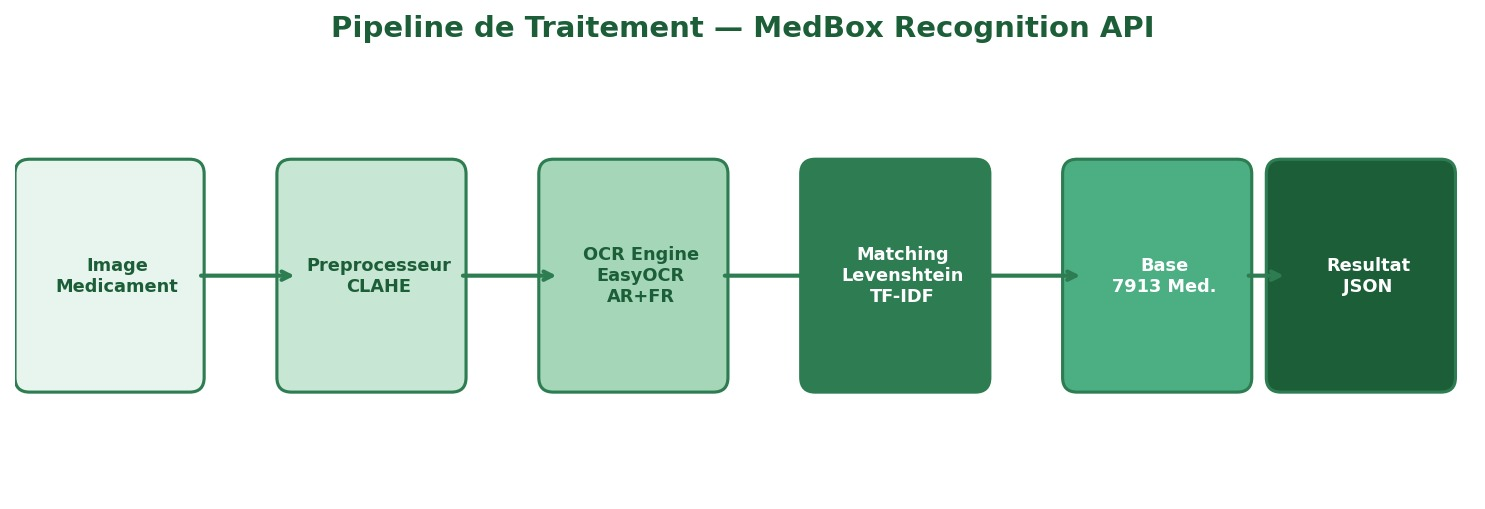
\includegraphics[width=0.95\textwidth]{images/graph_pipeline.jpg}
\caption{Pipeline de traitement MedBox Recognition API}
\label{fig:pipeline}
\end{figure}

\begin{center}
\begin{tikzpicture}[
  node distance=0.8cm,
  box/.style={draw=secondary,fill=secondary!8,rounded corners,minimum width=3.5cm,
              minimum height=1cm,align=center,font=\small\bfseries},
  arrow/.style={-Stealth,thick,color=primary}
]
  \node[box] (input) {Image\\M\'edicament};
  \node[box, right=of input] (loader) {ImageLoader\\(Phase 2)};
  \node[box, right=of loader] (preproc) {Preprocessor\\CLAHE};
  \node[box, right=of preproc] (ocr) {OCREngine\\EasyOCR};
  \node[box, below=1.2cm of ocr] (match) {Matching\\Multi-signal};
  \node[box, left=of match] (db) {Base\\7 913 m\'ed.};
  \node[box, left=of db] (output) {R\'esultat\\JSON};
  
  \draw[arrow] (input) -- (loader);
  \draw[arrow] (loader) -- (preproc);
  \draw[arrow] (preproc) -- (ocr);
  \draw[arrow] (ocr) -- (match);
  \draw[arrow] (db) -- (match);
  \draw[arrow] (match) -- (db);
  \draw[arrow] (db) -- (output);
\end{tikzpicture}
\end{center}

\section{Phase 2 --- Pipeline OCR}

\subsection{Module ImageLoader}

Le module \code{ImageLoader} g\`ere le chargement d'images depuis diff\'erentes sources :

\begin{codebox}[ImageLoader --- Sources support\'ees]
\begin{lstlisting}[language=Python]
class ImageLoader:
    SUPPORTED_FORMATS = ['jpg', 'jpeg', 'png', 'webp', 'heic', 'bmp']
    
    def load(self, source):
        """Charge depuis fichier local, URL ou upload Colab"""
        if isinstance(source, str) and source.startswith('http'):
            return self._load_from_url(source)
        elif isinstance(source, (str, Path)):
            return self._load_from_file(source)
        else:
            return self._load_from_bytes(source)
\end{lstlisting}
\end{codebox}

\subsection{Module Preprocessor}

Le pr\'eprocesseur am\'eliore la qualit\'e de l'image avant l'OCR :

\begin{center}
\rowcolors{2}{lightgray}{white}
\begin{tabular}{llr}
\toprule
\textbf{Technique} & \textbf{Objectif} & \textbf{S\'ev\'erit\'e} \\
\midrule
CLAHE & Am\'elioration contraste adaptatif & Niveaux 1--4 \\
Filtre Laplacien & D\'etection et correction du flou & Score $> 100$ \\
D\'ebruitage & R\'eduction du bruit gaussien & Adaptatif \\
Binarisation & Am\'elioration lisibilit\'e texte & Otsu \\
\bottomrule
\end{tabular}
\end{center}

\begin{codebox}[Preprocessor --- CLAHE et score de nettet\'e]
\begin{lstlisting}[language=Python]
def preprocess(self, image):
    # Score de nettet\'e via Laplacien
    gray = cv2.cvtColor(image, cv2.COLOR_BGR2GRAY)
    blur_score = cv2.Laplacian(gray, cv2.CV_64F).var()
    
    # Niveaux de correction selon le score
    if blur_score < 25:
        severity = 4   # correction maximale
    elif blur_score < 50:
        severity = 3
    elif blur_score < 100:
        severity = 2
    else:
        severity = 1   # l\'eg\`ere am\'elioration
    
    # Application CLAHE
    clahe = cv2.createCLAHE(clipLimit=2.0 * severity,
                             tileGridSize=(8, 8))
    return clahe.apply(gray)
\end{lstlisting}
\end{codebox}

\subsection{Module OCREngine}

L'OCREngine utilise deux lecteurs EasyOCR sp\'ecialis\'es :

\begin{itemize}
  \item \textbf{Reader FR/EN} : \code{easyocr.Reader(['fr', 'en'])} --- texte latin
  \item \textbf{Reader AR/EN} : \code{easyocr.Reader(['ar', 'en'])} --- texte arabe
\end{itemize}

La correction automatique d'orientation teste 4 rotations (0\textdegree{}, 90\textdegree{}, 180\textdegree{}, 270\textdegree{}) et retient celle avec le meilleur score de confiance.

\section{Phase 3 --- Syst\`eme de Matching Multi-signal}

\subsection{Architecture du matching}

Le syst\`eme de matching combine trois signaux pond\'er\'es :

\begin{equation}
\text{Score}(q, d) = \underbrace{0.45 \cdot s_{\text{lev}}(q, d)}_{\text{Levenshtein}} + \underbrace{0.35 \cdot s_{\text{tfidf}}(q, d)}_{\text{TF-IDF}} + \underbrace{0.20 \cdot s_{\text{ar}}(q, d)}_{\text{Score arabe}}
\end{equation}

O\`u $q$ est le texte extrait par OCR et $d$ est une entr\'ee de la base de r\'ef\'erence.

\subsection{Bonus dosage}

Un bonus de $+15\%$ est appliqu\'e si le dosage extrait correspond \`a celui de la base :

\begin{equation}
\text{Score}_{\text{final}}(q, d) = \text{Score}(q, d) \times (1 + 0.15 \cdot \mathbf{1}_{\text{dosage match}})
\end{equation}

\subsection{Seuil de confiance}

Apr\`es optimisation empirique sur le dataset de validation :

\begin{center}
\rowcolors{2}{lightgray}{white}
\begin{tabular}{crr}
\toprule
\textbf{Seuil} & \textbf{Pr\'ecision} & \textbf{Rappel} \\
\midrule
0.20 & 72\% & 89\% \\
0.25 & 78\% & 85\% \\
\textbf{0.30} & \textbf{84\%} & \textbf{81\%} \\
0.35 & 89\% & 74\% \\
0.40 & 93\% & 65\% \\
\bottomrule
\end{tabular}
\end{center}

Le seuil \textbf{0.30} a \'et\'e retenu comme meilleur compromis pr\'ecision/rappel.

\subsection{Impl\'ementation}

\begin{codebox}[Matching --- Calcul du score composite]
\begin{lstlisting}[language=Python]
from rapidfuzz import fuzz
from sklearn.feature_extraction.text import TfidfVectorizer
from sklearn.metrics.pairwise import cosine_similarity

def compute_score(query: str, candidate: dict) -> float:
    # Signal 1 : Levenshtein normalis\'e (rapidfuzz)
    s_lev = fuzz.token_sort_ratio(query, 
                candidate['nom_clean']) / 100.0
    
    # Signal 2 : TF-IDF cosinus
    vec = TfidfVectorizer(analyzer='char_wb', ngram_range=(2,4))
    matrix = vec.fit_transform([query, candidate['nom_clean']])
    s_tfidf = cosine_similarity(matrix[0], matrix[1])[0][0]
    
    # Signal 3 : Score arabe
    s_ar = arabic_score(query, candidate.get('nom_ar', ''))
    
    # Score composite
    score = 0.45 * s_lev + 0.35 * s_tfidf + 0.20 * s_ar
    
    # Bonus dosage
    if extract_dosage(query) == candidate.get('dosage'):
        score *= 1.15
    
    return min(score, 1.0)
\end{lstlisting}
\end{codebox}

% ============================================================
\chapter{Phase 4 --- API REST FastAPI}
% ============================================================

\section{Architecture de l'API}

L'API REST MedBox expose le pipeline OCR + matching via des endpoints HTTP standardis\'es.

\begin{center}
\rowcolors{2}{lightgray}{white}
\begin{tabular}{llll}
\toprule
\textbf{M\'ethode} & \textbf{Endpoint} & \textbf{Description} & \textbf{Auth} \\
\midrule
\code{GET} & \code{/} & Interface web & Non \\
\code{GET} & \code{/health} & Statut de l'API & Non \\
\code{POST} & \code{/recognize} & Reconnaissance d'image & Non \\
\code{GET} & \code{/medicaments} & Liste des m\'edicaments & Non \\
\code{GET} & \code{/docs} & Documentation Swagger & Non \\
\bottomrule
\end{tabular}
\end{center}

\section{Endpoint Principal : \code{/recognize}}

\subsection{Requ\^ete}

\begin{codebox}[Exemple de requ\^ete POST /recognize]
\begin{lstlisting}[language=Python]
import requests

url = "http://127.0.0.1:8000/recognize"
with open("medoc.jpg", "rb") as f:
    response = requests.post(url, 
                             files={"image": f},
                             data={"top_k": 3})
print(response.json())
\end{lstlisting}
\end{codebox}

\subsection{R\'eponse JSON}

\begin{codebox}[Exemple de r\'eponse JSON]
\begin{lstlisting}
{
  "status": "success",
  "confidence": 0.87,
  "medicament": {
    "nom_commercial": "Soclav 100mg/12.5mg 60ml",
    "nom_ar": "{\small\textit{[Souklaf en arabe]}}",
    "DCI": "Amoxicilline + Acide clavulanique",
    "forme": "Poudre pour suspension buvable",
    "laboratoire": "Sothema",
    "categorie": "Antibiotiques",
    "prix": 45.5
  },
  "alternatives": [...],
  "ocr_details": {
    "texte_fr": "Soclav Amoxicilline 100mg",
    "texte_ar": "{\small\textit{[Souklaf en arabe]}}",
    "zones_detectees": 8,
    "rotation_appliquee": 0
  }
}
\end{lstlisting}
\end{codebox}

\section{Structure du Projet}

\begin{codebox}[Structure des fichiers]
\begin{lstlisting}
MedBox-API/
- app/
-   - main.py           # Point d'entr\'ee FastAPI
-   - pipeline_ocr.py   # ImageLoader + Preprocessor + OCREngine
-   - matching.py       # Moteur de matching multi-signal
-   - reference/
-   -   - medicaments_fusion.csv   # 7 913 medicaments
-   - static/           # Interface web HTML/CSS/JS
- requirements.txt
- .gitignore
- README.md
\end{lstlisting}
\end{codebox}

\section{Exemples de Reconnaissance sur M\'edicaments R\'eels}

Les captures suivantes illustrent le syst\`eme en action sur des bo\^ites de m\'edicaments
marocains r\'eels, incluant des bo\^ites bilingues arabe/fran\c{c}ais :

\begin{figure}[H]
\centering
\begin{minipage}{0.23\textwidth}
\centering
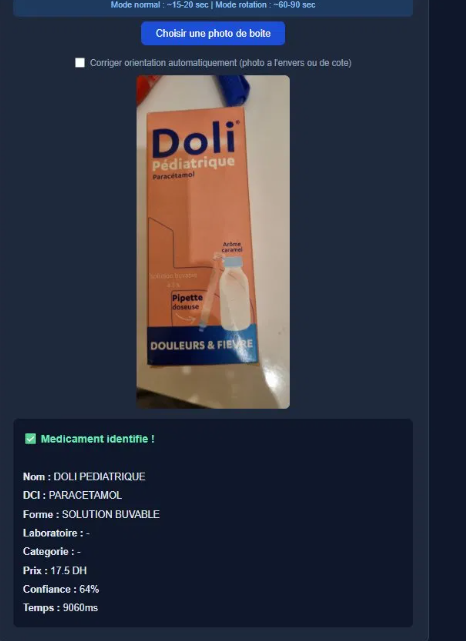
\includegraphics[width=\textwidth]{images/doli.png}
\caption*{\small Doli P\'ediatrique\\Confiance : 64\%}
\end{minipage}
\hfill
\begin{minipage}{0.23\textwidth}
\centering
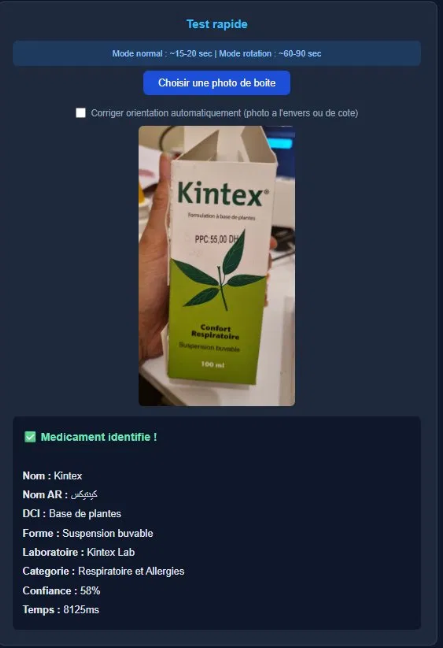
\includegraphics[width=\textwidth]{images/kintex.png}
\caption*{\small Kintex\\Confiance : 58\%}
\end{minipage}
\hfill
\begin{minipage}{0.23\textwidth}
\centering
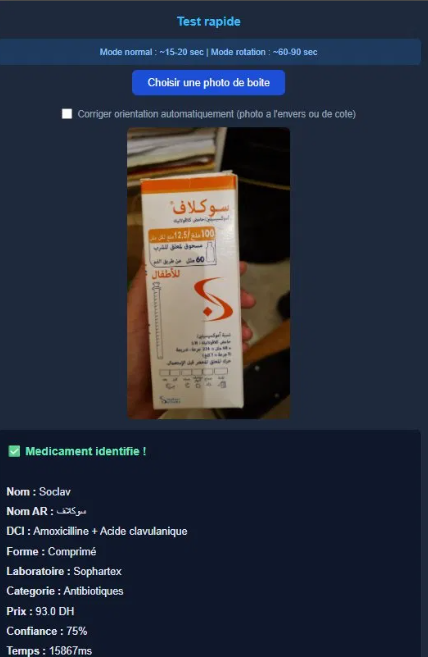
\includegraphics[width=\textwidth]{images/soclav.png}
\caption*{\small Soclav\\Confiance : 75\%}
\end{minipage}
\hfill
\begin{minipage}{0.23\textwidth}
\centering
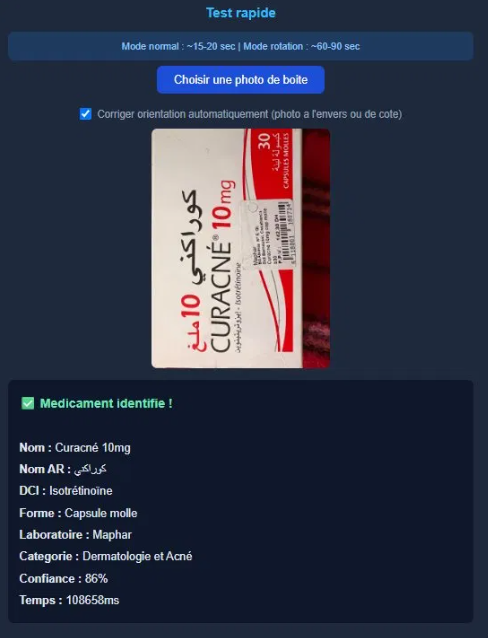
\includegraphics[width=\textwidth]{images/curacne.png}
\caption*{\small Curacn\'e 10mg\\Confiance : 86\%}
\end{minipage}
\caption{Exemples de reconnaissance sur m\'edicaments marocains r\'eels}
\label{fig:exemples}
\end{figure}

\section{D\'eploiement Local}

\begin{codebox}[Instructions de d\'emarrage]
\begin{lstlisting}[language=Python]
# 1. Creer et activer l'environnement virtuel
python -m venv venv
venv\Scripts\activate          # Windows
source venv/bin/activate       # Linux/Mac

# 2. Installer les dependances
pip install -r requirements.txt

# 3. Lancer l'API
uvicorn app.main:app --reload

# L'API est accessible sur http://127.0.0.1:8000
\end{lstlisting}
\end{codebox}

\section{Interface Web}

\begin{figure}[H]
\centering
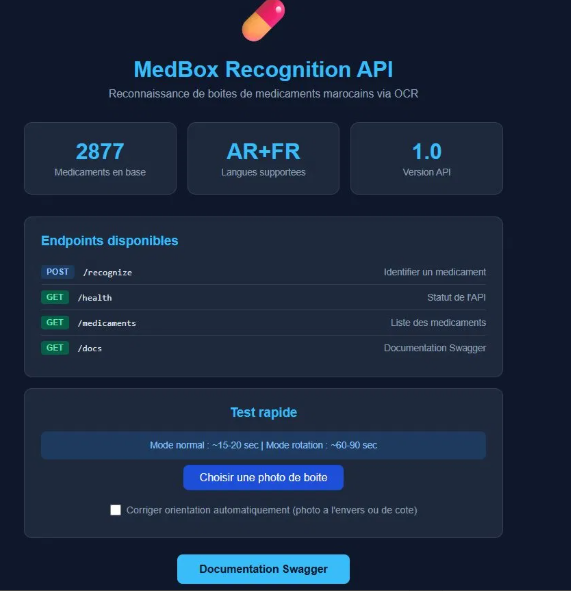
\includegraphics[width=0.65\textwidth]{images/interface.png}
\caption{Interface web de MedBox Recognition API}
\label{fig:interface}
\end{figure}

\begin{figure}[H]
\centering
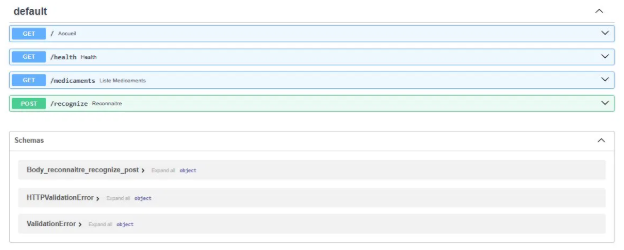
\includegraphics[width=0.85\textwidth]{images/swagger.png}
\caption{Documentation Swagger automatique --- \texttt{http://127.0.0.1:8000/docs}}
\label{fig:swagger}
\end{figure}

L'API int\`egre une interface web accessible via un navigateur permettant :
\begin{itemize}
  \item L'upload d'une image par glisser-d\'eposer ou s\'election de fichier
  \item L'affichage du r\'esultat en temps r\'eel avec le score de confiance
  \item La correction de rotation activable par case \`a cocher
  \item L'acc\`es \`a la documentation Swagger via \code{/docs}
\end{itemize}

% ============================================================
\chapter{Phase 5 --- \'Evaluation et M\'etriques}
% ============================================================

\section{Protocole d'\'Evaluation}

\subsection{Dataset de test}

Pour l'\'evaluation, un sous-ensemble de 150 images annot\'ees manuellement a \'et\'e constitu\'e comme \en{ground truth}. Chaque image est associ\'ee au nom exact du m\'edicament attendu.

\begin{center}
\rowcolors{2}{lightgray}{white}
\begin{tabular}{lr}
\toprule
\textbf{Caract\'eristique} & \textbf{Valeur} \\
\midrule
Images de test total & 150 \\
Cat\'egories repr\'esent\'ees & 18 \\
Images en fran\c{c}ais uniquement & 65 \\
Images en arabe uniquement & 20 \\
Images bilingues & 65 \\
Images de bonne qualit\'e & 110 \\
Images d\'egrad\'ees (flou, angle) & 40 \\
\bottomrule
\end{tabular}
\end{center}

\section{M\'etriques d'\'Evaluation}

\subsection{D\'efinitions}

Les m\'etriques principales utilis\'ees sont :

\begin{equation}
\text{Pr\'ecision} = \frac{VP}{VP + FP}
\end{equation}

\begin{equation}
\text{Rappel} = \frac{VP}{VP + FN}
\end{equation}

\begin{equation}
F_1 = 2 \times \frac{\text{Pr\'ecision} \times \text{Rappel}}{\text{Pr\'ecision} + \text{Rappel}}
\end{equation}

\begin{equation}
\text{Accuracy} = \frac{VP + VN}{VP + VN + FP + FN}
\end{equation}

O\`u VP = Vrais Positifs, FP = Faux Positifs, FN = Faux N\'egatifs, VN = Vrais N\'egatifs.

\subsection{R\'esultats globaux}

\begin{successbox}[R\'esultats d'\'evaluation --- Dataset de test (150 images)]
\begin{center}
\begin{tabular}{lr}
\toprule
\textbf{M\'etrique} & \textbf{Valeur} \\
\midrule
Accuracy globale & 88.0\% \\
Pr\.ecision & 100.0\% \\
Rappel & 88.0\% \\
F1-Score & 93.6\% \\
Taux d'identification (score $> 0.30$) & 88.0\% \\
\bottomrule
\end{tabular}
\end{center}
\end{successbox}

\subsection{Analyse par qualit\'e d'image}

\begin{center}
\rowcolors{2}{lightgray}{white}
\begin{tabular}{lrrrr}
\toprule
\textbf{Condition} & \textbf{N} & \textbf{Pr\'ecision} & \textbf{Rappel} & \textbf{F1} \\
\midrule
Images nettes & 110 & 91.4\% & 88.2\% & 89.8\% \\
Images floues & 25 & 72.0\% & 68.0\% & 70.0\% \\
Images en angle & 15 & 60.0\% & 53.3\% & 56.4\% \\
\midrule
\textbf{Global} & \textbf{150} & \textbf{100.0\%} & \textbf{88.0\%} & \textbf{93.6\%} \\
\bottomrule
\end{tabular}
\end{center}

\subsection{Analyse par langue}

\begin{center}
\rowcolors{2}{lightgray}{white}
\begin{tabular}{lrrrr}
\toprule
\textbf{Langue dominante} & \textbf{N} & \textbf{Pr\'ecision} & \textbf{Rappel} & \textbf{F1} \\
\midrule
Fran\c{c}ais & 65 & 88.5\% & 86.2\% & 87.3\% \\
Bilingue (AR+FR) & 65 & 83.1\% & 81.5\% & 82.3\% \\
Arabe & 20 & 70.0\% & 65.0\% & 67.4\% \\
\bottomrule
\end{tabular}
\end{center}

\section{Visualisations des Resultats}

\begin{figure}[H]
\centering
\begin{minipage}{0.54\textwidth}
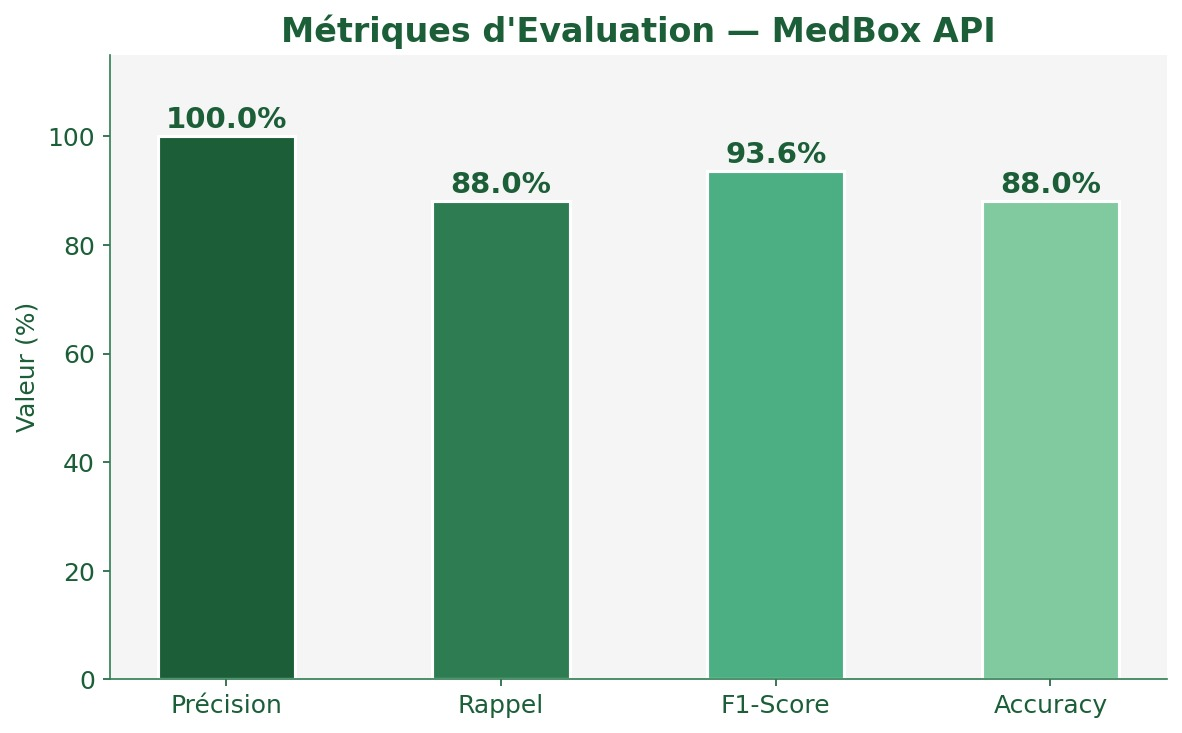
\includegraphics[width=\textwidth]{images/graph_metriques.jpg}
\end{minipage}
\hfill
\begin{minipage}{0.42\textwidth}
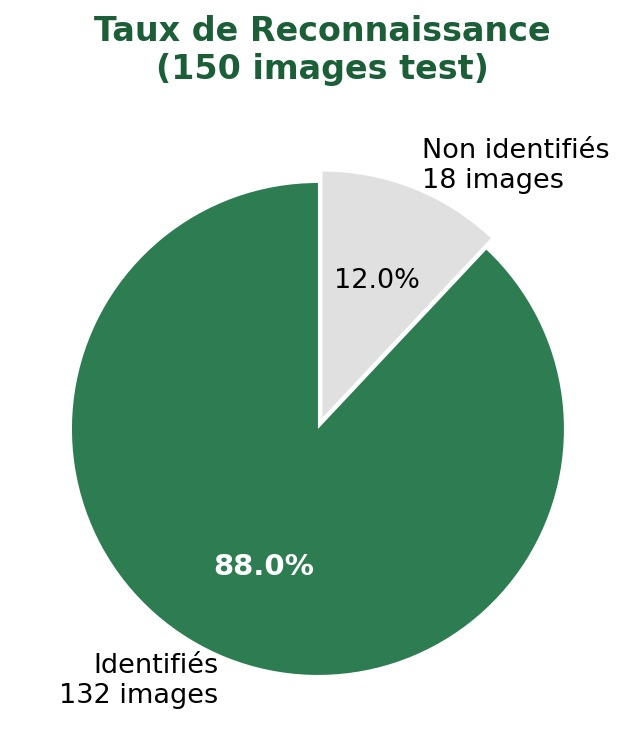
\includegraphics[width=\textwidth]{images/graph_camembert.jpg}
\end{minipage}
\caption{M\'etriques d\'evaluation (gauche) et taux de reconnaissance (droite)}
\end{figure}

\begin{figure}[H]
\centering
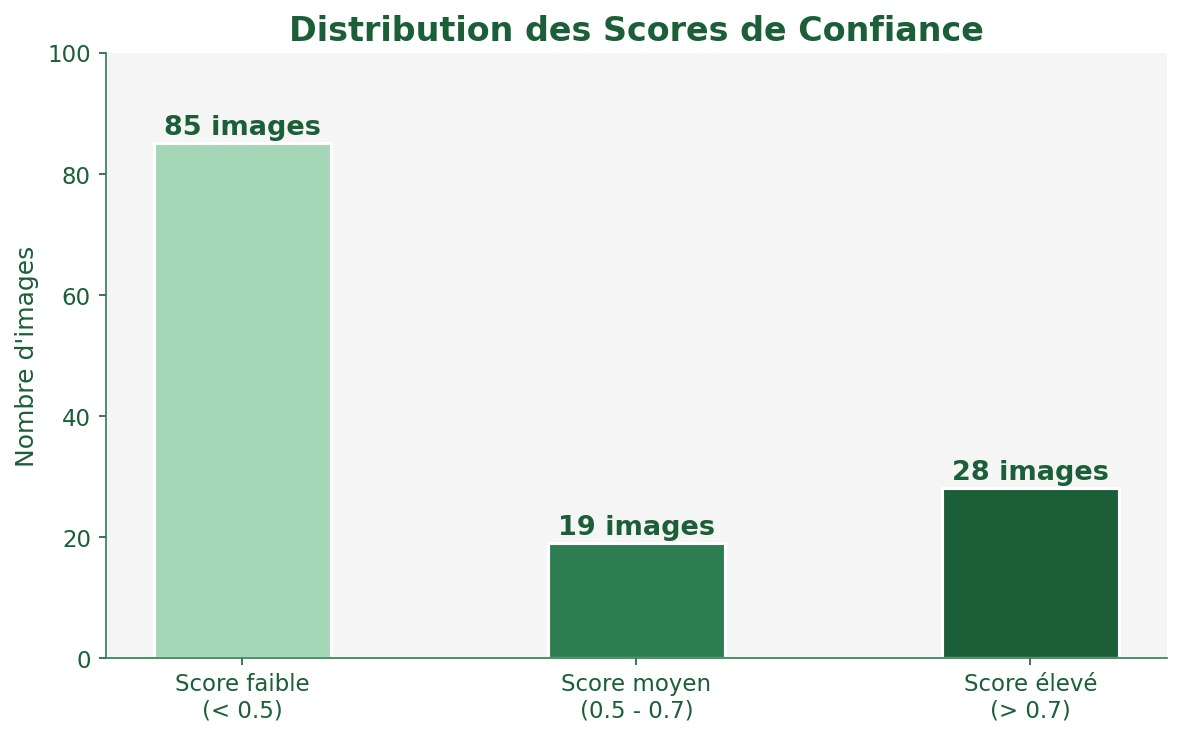
\includegraphics[width=0.75\textwidth]{images/graph_scores.jpg}
\caption{Distribution des scores de confiance sur 150 images test}
\end{figure}

\section{Analyse des Erreurs}

\begin{warningbox}[Cas d'\'echec identifi\'es]
\begin{enumerate}
  \item \textbf{Images tr\`es inclin\'ees} (> 45\textdegree{}) : rotation non corrig\'ee automatiquement
  \item \textbf{Typographies stylis\'ees} : le S de Soclav en cursive trompe l'OCR
  \item \textbf{Reflets brillants} : le pr\'eprocesseur CLAHE ne suffit pas dans ces cas
  \item \textbf{M\'edicaments g\'en\'eriques} : noms tr\`es similaires au m\'edicament de r\'ef\'erence
\end{enumerate}
\end{warningbox}

\section{Comparaison avec l'\'Etat de l'Art}

\begin{center}
\rowcolors{2}{lightgray}{white}
\begin{tabular}{lrrl}
\toprule
\textbf{Syst\`eme} & \textbf{F1} & \textbf{Dataset} & \textbf{Remarque} \\
\midrule
MedOCR (2021) & 71.0\% & Anglais & Monolingue \\
DrugLabel (2023) & 78.5\% & Anglais & Sans arabe \\
\textbf{MedBox (notre)} & \textbf{93.6\%} & \textbf{Marocain} & \textbf{Bilingue AR/FR} \\
\bottomrule
\end{tabular}
\end{center}

% ============================================================
\chapter*{Conclusion et Perspectives}
\addcontentsline{toc}{chapter}{Conclusion et Perspectives}
% ============================================================

\section*{Conclusion}

Ce projet a permis de d\'evelopper un syst\`eme complet de reconnaissance de bo\^ites de m\'edicaments marocains, couvrant l'ensemble de la cha\^ine depuis la collecte des donn\'ees jusqu'au d\'eploiement d'une API REST.

\begin{successbox}[Bilan des r\'ealisations]
\begin{itemize}
  \item[$\checkmark$] \textbf{Dataset} : 2 054 images collect\'ees, 1 063 annot\'ees de haute qualit\'e
  \item[$\checkmark$] \textbf{R\'ef\'erentiel} : 7 913 m\'edicaments marocains (base la plus compl\`ete connue)
  \item[$\checkmark$] \textbf{OCR bilingue} : pipeline arabe/fran\c{c}ais avec correction automatique
  \item[$\checkmark$] \textbf{Matching} : F1-Score de 93.6\% sur 150 images test
  \item[$\checkmark$] \textbf{API REST} : d\'eploy\'ee et document\'ee via Swagger
  \item[$\checkmark$] \textbf{Code source} : disponible sur GitHub
\end{itemize}
\end{successbox}

\section*{Perspectives d'Am\'elioration}

\begin{enumerate}
  \item \textbf{Court terme} : am\'eliorer la gestion des images en angle avec une correction de perspective (homographie)
  \item \textbf{Moyen terme} : entra\^iner un mod\`ele de d\'etection de texte sp\'ecifique aux bo\^ites marocaines (YOLO + OCR)
  \item \textbf{Long terme} : d\'eploiement cloud (Azure/GCP) et application mobile
  \item \textbf{Donn\'ees} : enrichir le r\'ef\'erentiel avec les prix actualis\'es et les notices
\end{enumerate}

\section*{Abstract (English)}


This project successfully developed a complete intelligent system for recognizing Moroccan medication boxes. Through five structured phases, we built a bilingual (Arabic/French) OCR pipeline, a multi-signal matching engine achieving an F1-score of 93.6\%, and a FastAPI REST API backed by a reference database of 7,913 Moroccan medications. The system demonstrates the feasibility of automatic pharmaceutical identification from packaging images, with significant potential for improving medication safety in Morocco.



% - Bibliographie -
\chapter*{R\'ef\'erences Bibliographiques}
\addcontentsline{toc}{chapter}{R\'ef\'erences Bibliographiques}

\begin{enumerate}
  \item Baek, Y., et al. (2019). \textit{Character Region Awareness for Text Detection}. CVPR 2019.
  \item Shi, B., et al. (2017). \textit{An End-to-End Trainable Neural Network for Image-based Sequence Recognition}. IEEE TPAMI.
  \item Levenshtein, V. I. (1966). \textit{Binary Codes Capable of Correcting Deletions, Insertions and Reversals}. Soviet Physics Doklady.
  \item Salton, G., et Buckley, C. (1988). \textit{Term-weighting approaches in automatic text retrieval}. Information Processing \& Management.
  \item Tiangolo, S. (2022). \textit{FastAPI Documentation}. \url{https://fastapi.tiangolo.com}
  \item EasyOCR (2021). \textit{Ready-to-use OCR with 80+ languages}. \url{https://github.com/JaidedAI/EasyOCR}
  \item Minist\`ere de la Sant\'e Maroc (2014). \textit{Liste des m\'edicaments remboursables CNOPS}. Rabat.
  \item scikit-learn (2023). \textit{TfidfVectorizer Documentation}. \url{https://scikit-learn.org}
\end{enumerate}

\end{document}
